\documentclass[a4paper,12pt]{article} 
\usepackage{german}
\usepackage[T1]{fontenc}
\usepackage[utf8]{inputenc}
\usepackage{graphicx}
\usepackage{float}
\usepackage[numbib]{tocbibind}
\usepackage{gensymb}
\begin{document}
\renewcommand\bibname{Referenzen}
\renewcommand\refname{Referenzen}

\begin{titlepage}
\author{Elena Noll\\
		Sven-Hendrik Haase}
\title{Erkennung von Toren beim RoboCup} 
\date{\today} 
\maketitle
\thispagestyle{empty}
\end{titlepage}

\tableofcontents

\newpage

\section{Einführung}
Diese Arbeit beschäftigt sich mit der Bilderkennung der Tore im RoboCup.
Diese ist genau wie z.B. die autonome Bewegung oder die Lokalisierung ein zentraler Punkt der Forschung.
Wichtig ist, dass der Roboter wissen muss nach was er eigentlich sucht. Das bedeutet, er muss wissen, welche Größe, welche Farbe und wleche Form das Tor hat, damit er es erkennen kann.
Wichtig ist dabei zu wissen, dass der RoboCup in verschiedenen Ligen
angeboten wird, die jeweils verschiedene Tore einsetzen. Dies wird später
genauer erläutert. Es werden zudem zwei von vielen möglichen Verfahren zur Erkennung
der Tore genauer vorgestellt.

\section{Tore im RoboCup}
Die Tore im RoboCup haben genau wie beim "normalen" Fussball mit menschlichen
Spielern die Funktion, Punkte zu werten.
Allgemein bestehen alle Tore im RoboCup unabhängig von der Liga genau wie normale Fußballtore aus zwei Pfosten, einer Latte und einem Netz. Die Tore werden auf der Torlinie mittig zentriert aufgestellt, sodass die Torlinie und die Latte parallel zueinander sind.

Der RoboCup besteht aus verschiedenen Ligen, die grob ihrer Größe nach
gestaffelt sind. In jeder Liga können die Tore eine unterschiedliche Größe sowie Farbe haben. Das Tor jeder Liga kann sich zudem jedes Jahr unabhängig von den
anderen Ligen verändern. Der allgemeine Gedanke hierbei ist, dass die
Anforderungen an die Roboter und somit die Teams jedes Jahr wachsen sollen und es jedes Jahr neue Herausforderungen geben soll. Ein Beispiel hierfür ist, dass im letzen Jahr durch in der SPL ersmals gleichfarbige Tore eingeführt wurden.
Dies erschwert die Schwirigkeit der Selbstlokalisation der Roboter erheblich.

\subsection{Middle Size League}

\begin{figure}[H]
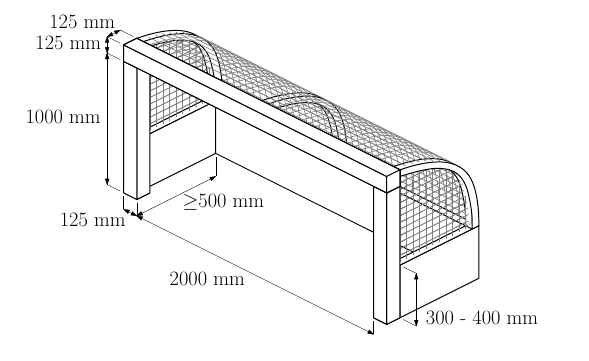
\includegraphics{middlesize-goal.png}
\caption{Tor in der Middle Size League}
\label{fig:goal-msl}
\end{figure}

Die Grafik zeigt die Maße an. Die Farbe beider Tore bei der Middle Size League ist seit einigen
Jahren weiss. Eine besondere Schwierigkeit bei der Bilderkennung stellt hierbei das ebenfalls
weisse Netz dar, welches
fälschlicherweise als Feldlinie erkannt werden könnte. Die Tore besitze eine geschlossene Form. Das
Netz ist solide und behält seine Form, was es von "echten" Netzen beim Fußball unterscheidet.


\subsection{Humanoid League}
\begin{figure}[H]
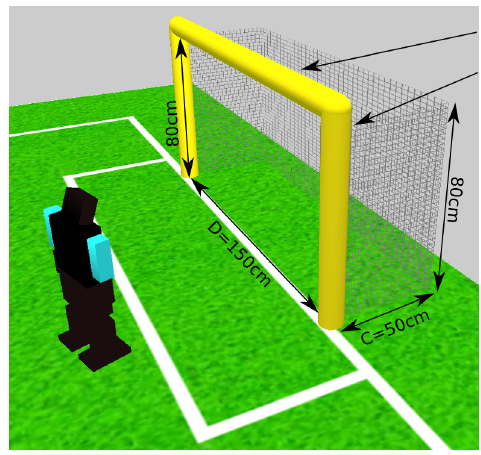
\includegraphics{humanoid-kidsize-goal.png}
\caption{Tor in der Kid Size Humanoid League}
\label{fig:goal-human-kid}
\end{figure}

\begin{figure}[H]
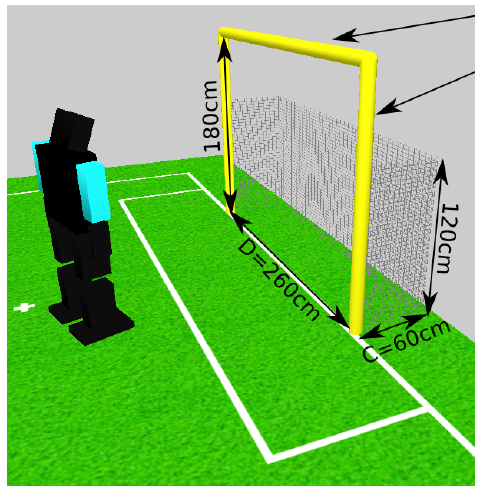
\includegraphics{humanoid-adultsize-goal.png}
\caption{Tor in der Adult Size Humanoid League}
\label{fig:goal-human-adult}
\end{figure}
Wie in den Grafiken dargestellt, gibt es für die beiden Größen der Humanoid League auch jeweils ein
passendes Tor. Anders als bei der Middle Size League sind die Torfarben jedoch unterschiedlich:
Eines ist blau, das andere ist gelb. Das Regelwerk von 2012 stellt in Aussicht, dass sich dies bald
ändern könnte. Hinter dem Tor befindet ein engmaschiges, solides Netz mit dunkler Farbe.

\subsection{Standard Platform League}
\begin{figure}[H]
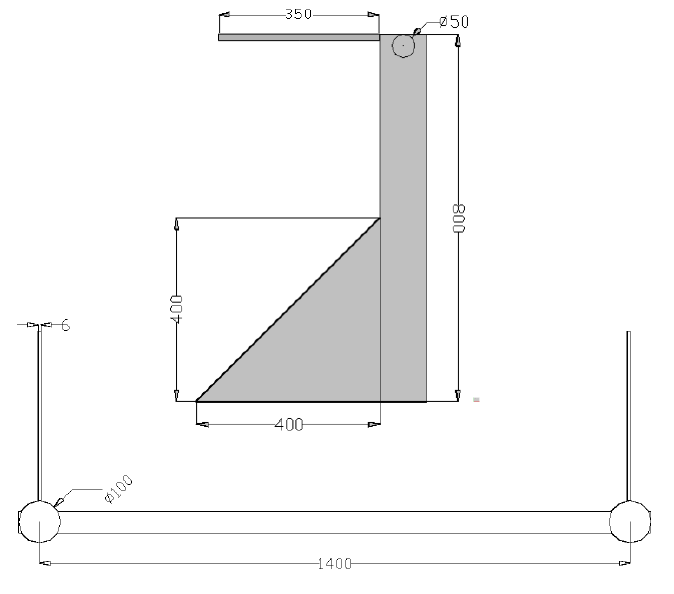
\includegraphics[scale=0.8]{spl-goal.png}
\caption{Tor in der Standard Platform League}
\label{fig:goal-spl}
\end{figure}
Bei den Toren der Standard Platform League fallen die zusätzlichen Keile an Torpfosten auf, die
sich nach hinten zur Befestigung des Netzes erstrecken. Diese Keile können zusätzlich bei der
Bildverarbeitung dazu benutzt werden, den Roboter sich lokalisieren zu lassen, da sie mehr
geometrische Informationen bieten, als ein einzelner Torpfosten. Zu bemerken ist auch, dass die
Farbe beider Tore seit 2012 auf gelb festgelegt ist.

\section{Bilderkennung}
Die optische Erkennung von Toren im RoboCup ist ein wichtiger Bestandteil des Wettbewerbs. Obwohl
Bilderkennung im Allgemeinen nichts Neues ist, ist das stetige Verbessern bestehender Verfahren und das
Finden neuer Methoden Teil fortlaufender Forschung. Die sich ständig ändernden Regeln des RoboCups
sorgen mitunter auch dafür, dass bestehende Algorithmen ihre Effektivität verlieren und jährlich
revisioniert werden müssen. In dieser Arbeit werden zwei von vielen Verfahren vorgestellt, da die
beiden Verfahren die unterschiedlichen Herangehensweisen gut veranschaulichen.

\subsection{Probleme}
Die allgemeinen Probleme, die es bei der Bilderkennung für Tore zu lösen gilt, sind aufgrund
der Umstände mannigfaltig: Durch die Mobilität des Roboters ändert sich die Perspektive ständig. Das
führt dazu, dass das Bild des Tores, welches der Roboter erhält, teilweise startk verzerrt wird. Es
kann beispielsweise vorkommen, dass der Roboter nur den unteren Teil eines einzigen Pfostens sieht.
Dies führt zu großen Probleme bei der Lokalisation anhand dieses Bildes alleine, sodass das der
optische Momenteindruck so nicht ausreicht, um festzustellen, wo sich der Roboter befindet. Das
optische System muss also in ein umfassenderes System eingebettet werden. Die mittlerweile teils
gleichfarbigen Tore kommen hierbei erschwerend hinzu. \\

Ein weiteres Probleme wurde bereits erwähnt: Tornetze können teilweise als Feldlinien erkannt
werden. Außerdem können Teile vom Tor verdeckt sein (z.B. von anderen Robotern) oder es könnten
Hindernisse in der Schussbahn stehen. Letzteres ist nicht direkt ein Problem der Torerkennung, aber
es ist damit eng verbunden, denn ein Torschussversuch kann nur erfolgreich sein, wenn der Schuss
nicht vorher blockiert wird. Der Roboter muss sich also bewusst sein, wie er sich positionieren
muss, damit ein Schussversuch gelingen kann. \\

Letztendlich muss die Lösung als Programm implementiert werden, welches auf der
verwendeten Hardware des Roboters lauffähig ist. Diese Hardware ist häufig
im Vergleich zu größeren Rechnern stark eingeschränkt, sodass die Lösung
gut optimiert werden muss. Dies kann als versteckte Schwierigkeit aufgefasst
werden, denn eine theoretische Lösung, die algorithmisch bzw. mathematisch 
perfekt ist, läuft wahrscheinlich unpraktikabel langsam auf einem RoboCup
Roboter.

\newpage
\subsection{Erkennung mittels geometrischer Relationen}
Bei diesem Verfahren, das die geometrischen Sturkturen der Elemente im RoboCup ausnutzt, werden
vier Schritte ausgeführt:
\begin{enumerate}
	\item Farbkalibrierung im YUV-Farbraum
	\item Farbsegmentierung
	\item Erkennung des Horizonts
	\item Extraktion der Torpfosten und Modellierung
\end{enumerate}

\subsubsection{Farbkalibrierung YUV-Farbraum}
Der YUV-Farbraum besteht aus drei Komponenten: Helligkeit und zwei Farbkomponenten.
Er wurde ursprünglich für das analoge Farbfernsehen eingesetzt.
Dies war aus zwei Gründen günstig: Zum einen war Kompatibilität zu alten
Graustufen-Fernsehern gewährleistet, da lediglich die beiden neuen Farbkomponenten
zum ursprünglichen Graustufenbild hinzukamen und zum anderen, da sich das menschliche
Auge in diesem Farbraum besonders Fehlertolerant verhält, sodass selbst bei
schlechten Lichtverhältnissen die wichtigen Details erkennbar sind.
Der letzte Punkte ist ausschlaggebend für die Verwendung in diesem 
Bilderkennungsverfahren, da auch Roboter von der seperaten
Helligkeitskomponente profitieren und besser bei wenig Licht arbeiten können.
\newpage
Die folgende Grafik zeigt, wie sich ein Bild im YUV-Farbraum zusammensetzt:
\begin{figure}[H]
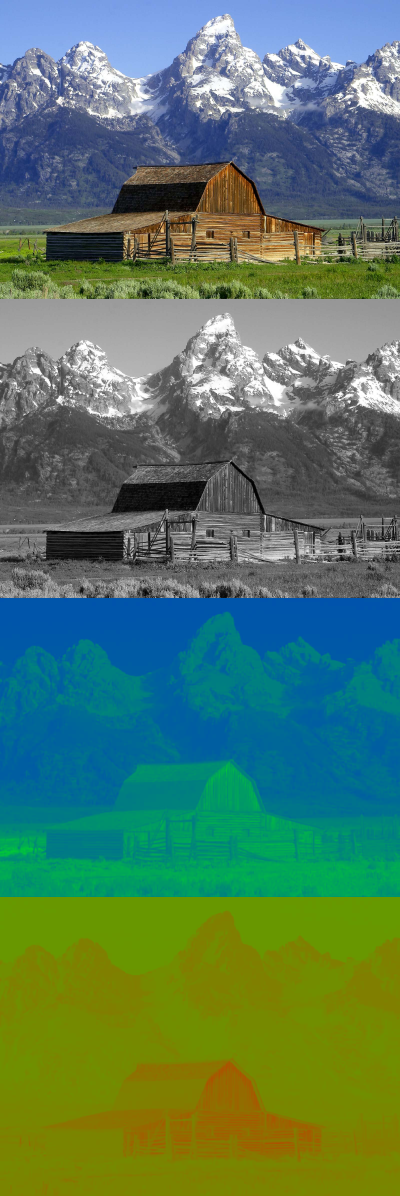
\includegraphics[scale=0.5]{Barn-yuv.png}
\caption{Beispiel eines Bildes im YUV-Farbraum}
\label{fig:yuv}
\end{figure}

\subsubsection{Farbsegmentierung}
Bei der Farbsegmentierung geht es darum, Bereiche ähnlicher Farbe in einem Bild
durch eine eindeutige Farbe zu markieren. Dies erleichtert die weitere
Verarbeitung dieses Bildes enorm, da alle gleichfarbigen Bereiche in der
Pixelmatrix nun den gleichen Wert haben. Wenn dieses Verfahren nicht angewendet
würde, wären die Farbwerte selbst auf einem guten Bild nie eindeutig, da sich
die Farbwerte sogar in einem Bild eines perfekt belichteten einfarbigen Gegenstandes
unterscheiden.

\newpage
Ein bekannter und einfacher Algorithmus für das Finden von Bereichen ähnlicher
Farbe ist der Region Growing-Algorithmus. Hierbei wird ein beliebiger Punkt in
einer Figur eines Bildes selektiert (manuell oder automatisch) und als Startpunkt
festgelegt. Die Farbwerte in dem Startpunkt werden festgestellt und gespeichert.
In der nächsten Iteration des Algorithmus wächst der selektierte Bereich ab 
Startpunkt um ein Pixel nach außen in alle Richtungen, solange der jeweilige 
neue Pixel einen Farbwer aufweist, der einen beliebigen Toleranzwert nicht 
übersteigt. Wenn der Toleranzwert an dieser Stelle überstiegen würde (z.B. durch
starke Farb- oder Helligkeitsunterschiede), dann wird an dieser Stelle nicht
weiter gewachsen. Dieser Algorithmus iteriert solange, bis es in einer Iteration
nicht mehr möglich ist, ein einziges Mal zu wachsen. Ab dann ist diese Fläche
zu ende markiert.
\\
Die folgende Grafik soll den Algorithmus veranschaulichen:
\begin{figure}[H]
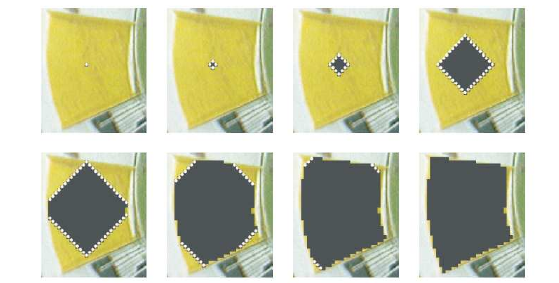
\includegraphics[scale=0.9]{region-growing.png}
\caption{Vorgang der Farbsegmentierungs-Algorithmus}
\label{fig:color-seg-algo}
\end{figure}

\newpage
Die folgende Grafik zeigt ein auf diese Weise markiertes Tor im RoboCup:
\begin{figure}[H]
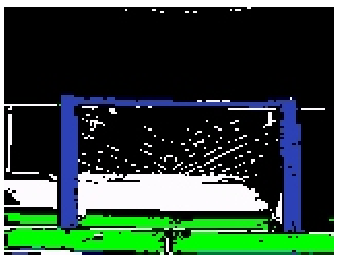
\includegraphics{segmented-view2.png}
\caption{Farbsegementiertes Bild eines RoboCup-Tores}
\label{fig:color-seg}
\end{figure}
Es ist einfach zu sehen, dass das gesamte Tor einfarbig blau markiert wurde,
wodurch die Weiterverarbeitung stark vereinfacht wird.

\newpage
Einige Programme existieren, um Robotern interaktiv verschiedene Farbflächen
beizubringen. Dies erleichtert die Schwellenwertfindung und lädt zu Experimenten
mit verschiedenen Lichtverhältnissen ein. Eines dieser Programme sieht so aus:
\begin{figure}[H]
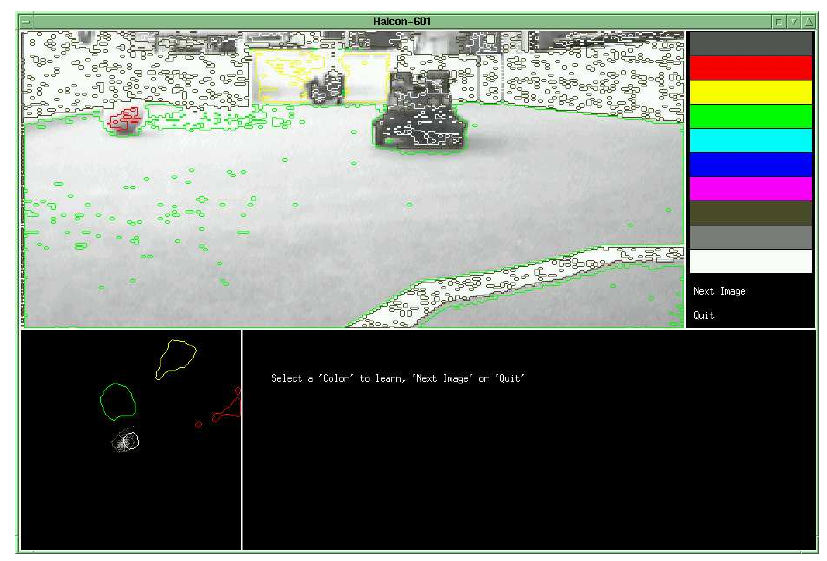
\includegraphics[scale=0.5]{training-tool.png}
\caption{Programm zur interaktiven Echtzeit-Farbsegmentierung}
\label{fig:color-seg-tool}
\end{figure}

Das Ergebnis mit diesem Programm sieht wie folgt aus:
\begin{figure}[H]
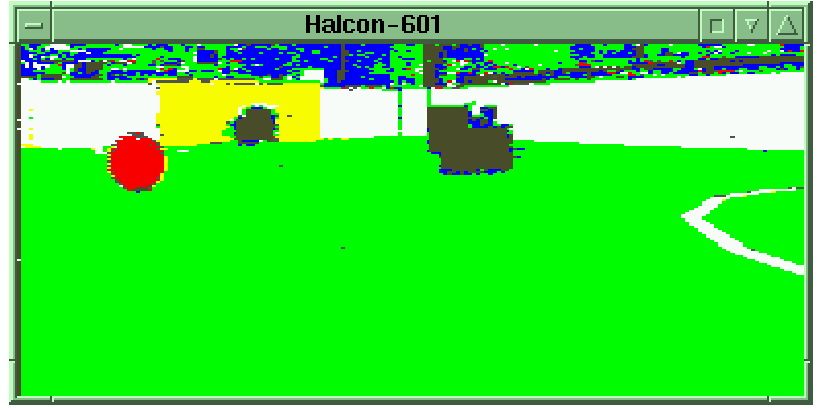
\includegraphics[scale=0.5]{segmented-view.png}
\caption{Segmentiertes Kamerabild}
\label{fig:color-seg-cam}
\end{figure}

\subsubsection{Erkennung des Horizons}
Als nächstes folgt die geometrische Erkennung, bei der sich zu Nutze gemacht
wird, dass alle Pixel oberhalb der Torlatte unbenötigte Informationen
darstellen. Deshalb wird die Torlatte als obere Grenze und Horizont 
festgelegt und das Bild darüber abgeschnitten. Zudem wird die Torlinie
erkannt und als unterer Horizone gewertet.
\begin{figure}[H]
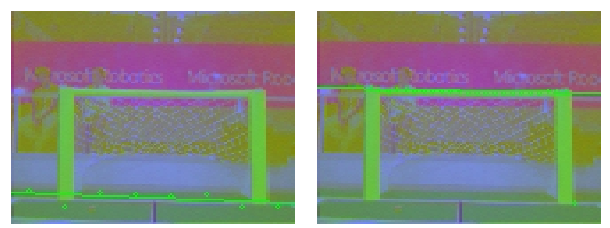
\includegraphics[scale=0.8]{geometric-plane.png}
\caption{Geometrische Horizonterkennung}
\label{fig:geom-horiz}
\end{figure}

\subsubsection{Extraktion der Torpfosten und Modellierung}
Mithilfe von Scanlinien wird das inzwischen markierte und eingeschränkte Tor
extrahiert und mittels Rechtecken modelliert.
\begin{figure}[H]
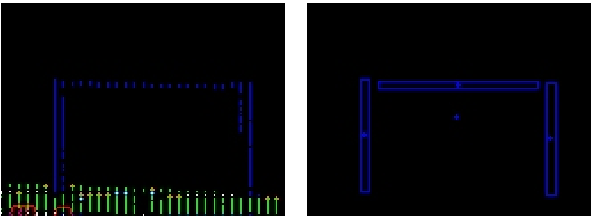
\includegraphics[scale=0.8]{goal-blobs.png}
\caption{Links: Extraktion; Rechts: Modellierung}
\label{fig:model}
\end{figure}

\subsubsection{Beispiele}
Nachfolgend ein paar anschauliche Beispiele der vier Schritte. Sie zeigen
besonders die Stabilität und Verlässlichkeit des Algorithmus selbst bei 
schlechten Bedingungen wie verdeckten Torpfosten und ungünstigen Perspektiven.
\begin{figure}[H]
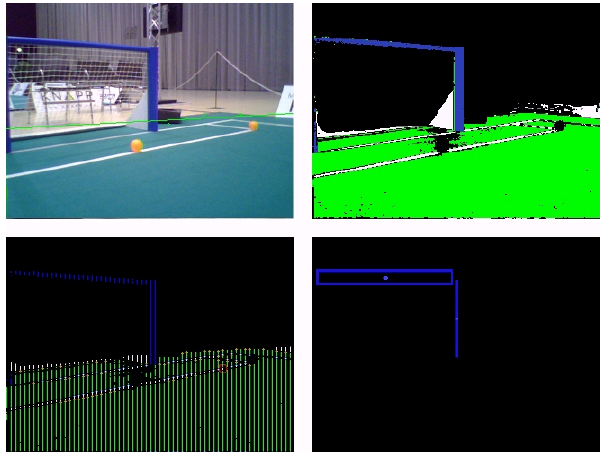
\includegraphics[scale=0.8]{example-detection1.png}
\caption{Beispiel des Verfahrens mit teils unsichtbarem Torpfosten}
\label{fig:example1}
\end{figure}

\begin{figure}[H]
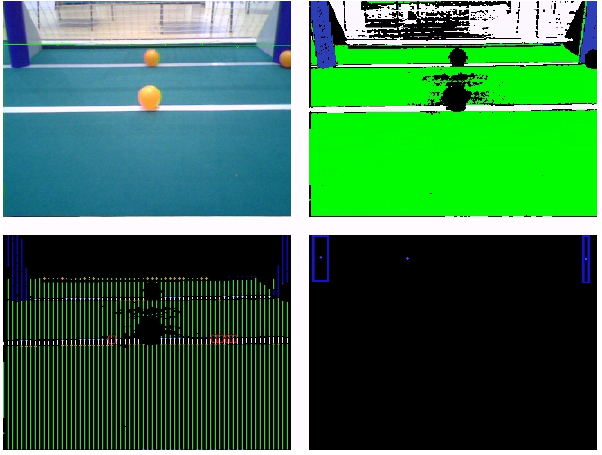
\includegraphics[scale=0.8]{example-detection2.png}
\caption{Beispiel des Verfahrens mit Bodenblick und wenig Torpfostenanteil im Bild}
\label{fig:example2}
\end{figure}

\begin{figure}[H]
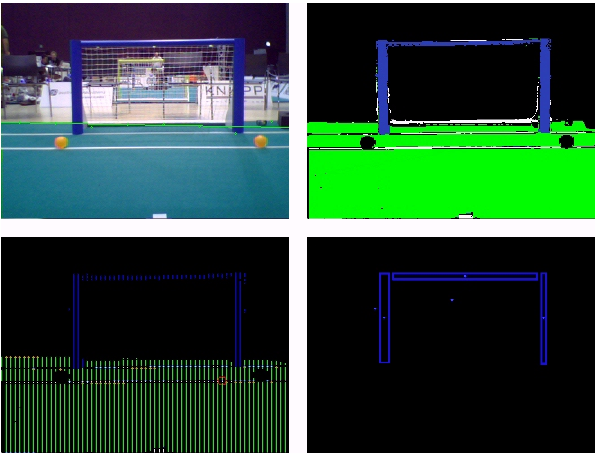
\includegraphics[scale=0.8]{example-detection3.png}
\caption{Beispiel des Verfahrens unter optimalen Bedingungen}
\label{fig:example3}
\end{figure}

\begin{figure}[H]
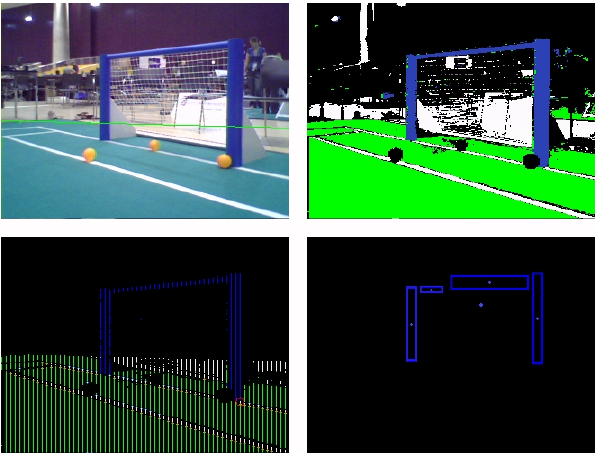
\includegraphics[scale=0.8]{example-detection4.png}
\caption{Beispiel des Verfahrens mit ungünstiger Perspektive}
\label{fig:example4}
\end{figure}

\subsection{Erkennung mittels Hough-Transformation}
Ein weiterer Weg zur Torerkennung im RoboCup ist die Hough-Transformation.
Die Hough-Transformation wurde 1962 von P.V.C. Hough entworfen und von Ihm unter dem Namen
„Method and Means for Recognizing Complex Patterns“ patentiert. Später wurde Sie von Duda und Hart weiterentwickelt und verbessert. \\
\\
Die Hough-Transformation stellt ein Verfahren zur Erkennung von beliebigen, vorgegebenen
geometrischen Strukturen in einem Gradientenbild dar. Angewendet wird dieses Verfahren
nicht nur im RoboCup sonder häufig auch zu industriellen Zwecken. Beispielsweise um bestimmte Arbeitsvorgänge von Maschinen zu automatisieren oder zu verbessern. \\
\\
Im Bezug auf die Torerkennung im RoboCup führt die Hough-Transformation alleine zu keinem
Ergebnis. Zur endgültigen Erkennung des Tores mittels der Hough-Transformation sind 4
wesentliche Schritte nötig. Hat der Roboter ein Bild eingefangen finden zunächst 2
Schritte statt, dieses Bild auf die Hough-Transformation vorzubereiten. Der erste Schritt
ist die Farbfilterung im HSV-Farbraum, der zweite Schritt ist die Anwendung eines
Eckenfilters zum Erkennen der Torkonturen. Erst danach ist das Bild so weit aufgearbeitet und die eigentliche Hough-Transformation kommt zum Einsatz um die Torsegmente zu erkennen. Zuletzt wird das entstandene Tormodell anhand von Eckpunkten modelliert und aufgespannt. Im folgenden werden die einzelnen Schritte genauer erläutert.

\subsubsection{Der HSV-Farbraum}
Im HSV-Farbraum werden Farben über drei Komponenten definiert.
Die H (Hue) Komponente beschreibt den Farbton, die S (Saturation) Komponente bestimmt wie satt bzw. blass die Farben dargestellt werden und mit der V Komponente kann die Helligkeit definiert werden.
\begin{figure}[H]
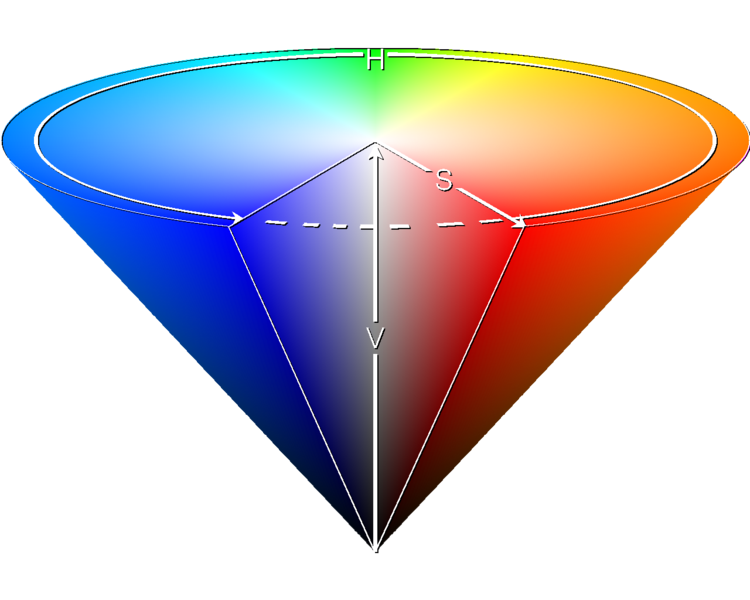
\includegraphics[scale=0.3]{hsv-farbraum.png}
\caption{HSV-Farbraum als Kegel}
\label{fig:hsv-farbraum}
\end{figure}

\paragraph{Farbfilterung im HSV-Farbraum}
\subparagraph{Farbfilterung}
Unter Farbfilterung versteht man ein Verfahren, das eine bestimmte Farbe in einem Bild erkennt und nur diese herausfiltert. Alles andere im Bild wird vernachlässigt und nach der Farbfilterung nicht mehr dargestellt.
\subparagraph{Warum Farbfilterung im HSV-Farbraum?}
Probleme bei der Farbfilterung entstehen dadurch, dass die Farbe des Tores z.B. durch unterschiedlichen Lichteinfall, Schatten oder Verschmutzung unterschiedlich wahrgenommen werden. Genau dort liegt der große Vorteil des HSV-Farbraumes. Ein Farbton kann unabhängig von Schwankungen der Helligkeit geprüft werden, indem man nur den Farbton zur Farbfilterung verwendet und die Sättigung und den Hellwert vernachlässigt. Somit ist die Farbprüfung unabhängig von Schattenbildungen, Schmutz oder Schwankung in der Intensität einer Lichtquelle möglich.
\begin{figure}[H]
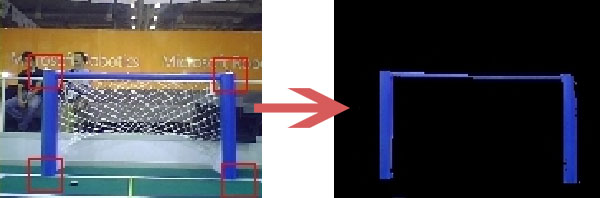
\includegraphics[scale=0.6]{farb-filterung.jpg}
\caption{Bild nach Anwendung der Farbfilterung im HSV-Farbraum}
\label{fig:farb-filterung}
\end{figure}

\subsubsection{Eckenfilter zum Erkennen von Torkonturen} 
Das Bild ist nach Anwendung des Farbfilters teilweise für die Hough-Transformation vorbereitet. Nun müssen nur noch mittels eines Eckenfilters die Torkonturen ausgearbeitet werden, da nur diese später relevant sind.

Das Erkennen der Konturen beruht auf der Tatsache, dass im Bereich einer Kontur eine sehr starke Helligkeits- bzw. Farbänderung vorliegt. In unserem Beispiel des blauen Tores, haben wir die blaue Farbe herausgefiltert und der Rest des Bildes wird schwarz dargestellt. Nun gehen wir mit Hilfe eines Algorithmus von einem blauen Pixel aus in eine beliebige Richtung. Solange, bis eine starke Farb- bzw. Helligkeitsveränderung festgestellt wird. An den Stellen, an denen eine Veränderung erkannt wird, muss eine Kante vorliegen. Die Kanten werden nachgezeichnet und als einfache Linien dargestellt. Nach der Durchführung der ersten beiden Schritte liegt uns nun ein segmentiertes Bild vor.
\begin{figure}[H]
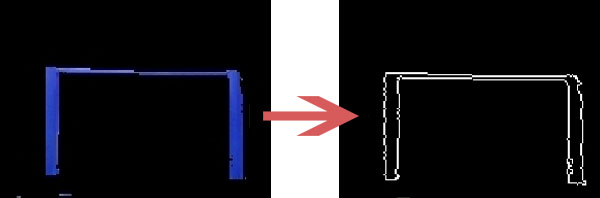
\includegraphics[scale=0.6]{eckenfilter.jpg}
\caption{Bild nach Anwendung des Eckenfilters}
\label{fig:eckenfilter}
\end{figure}
\subsubsection{Hough-Transformation zum Erkennen der Torsegmente}
Nachdem das Bild nun fertig vorverarbeitet ist, können wir zum eigentlichen Schritt der Hough-Transformation selbst kommen. Ziel dieses Verfahrens ist es wie Anfangs schon erwähnt eine vorgegebene Referenzstruktur in einem Bild zu erkennen. In unserem Beispiel ist die Referenzstruktur eine Gerade, da das Tor aus Geraden (den zwei Pfosten und der Latte) besteht.

Geraden werden oft wie in der Schule schon gelernt durch die Form 
\(y = m*x + b\) dargestellt. Die Idee hinter der Hough-Transformation ist es alle Punkte in einem Bild in einen anderen Raum, der als Dualraum oder auch Hough-Raum bezeichnet wird zu transformieren. Dazu müssen zunächst geeignete Parameter für eine Gerade gefunden werden. Dies ist in der Form
\(y = m*x + b\) nur bedingt möglich. Aus diesem Grund wandelt man die Gerade erst in die Hessesche Normalform um. Liegt uns die Gerade in der Form 
\(d = x*cos(\alpha) + y*sin(\alpha)\) vor wählen wir als unsere beiden Parameter den Abstand d und den Winkel \(\alpha\). Diese beiden Parameter dienen uns nun dazu, den neuen Raum aufzuspannen. Der Winkel wird die neue x-Achse und der Abstand die neue y-Achse wie auch in Abbildung \ref{fig:hough1} zu sehen ist.
\begin{figure}[H]
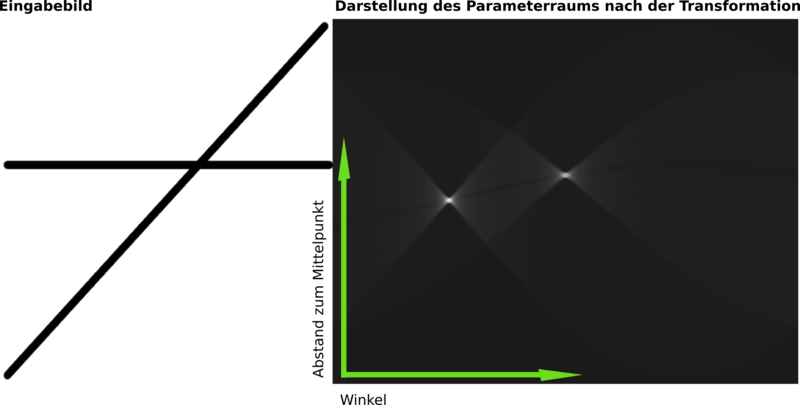
\includegraphics[scale=0.45]{hough1.png}
\caption{Beispiel für eine Hough-Transformation}
\label{fig:hough1}
\end{figure}
Nachdem geeignete Parameter gewählt wurden. Werden alle Punkte im Ausgangsbild in den neuen Raum transformiert. Dies funktioniert folgendermaßen. Es wird ein Punkt ausgewählt und von diesem aus für alle möglichen Winkel der dazugehörige Abstand berechnet. Für alle Winkel und die dazugehörigen Abstände trägt man die so entstehenden Punkte im Dualraum ein. Dadurch entsteht für jeden Punkt im Ausgangsbild eine Kurve im Dualraum. Jede dieser Kurven in unserem Hough-Raum repräsentiert also einen Punkt im Ausgangsbild. Der Hough-Algorithmus überträgt nach eben beschriebenem Verfahren alle Punkte in den Dualraum. Das Entscheidende ist nun, dass alle Kurven, die Punkte einer Geraden im Ausgangsbild repräsentieren sich in einem Punkt im Dualraum schneiden. Finden wir im Hough-Raum also solche Schnittstellen wissen wir, dass an diesen Stellen eine Gerade im Originalbild vorliegt. Dies ist auch in Abbildung 1.4 zu sehen. Die Kurven im rechten Bild repräsentieren Punkte im linken Bild. An zwei Stellen im linken Bild sieht man hellere Punkte, das sind die beiden Punkte an denen sich die Kurven schneiden und somit die Punkte, an denen Geraden vorliegen.\\
\\
Anders kann man das Transformieren in den Dualraum auch als Matrix und nicht grafisch darstellen. Dies Funktioniert genau wie oben beschrieben, nur dass man für alle Winkel und die dazugehörigen Abstände nicht ein Punkt im neuen Dualraum einträgt sondern in eine Matrix. Diesmal entsprechen die Spalten der Matrix den Winkeln und die Zeilen den Abständen. Ein Eintrag in der Matrix bedeutet, den Wert in der Matrix an dieser Stelle um Eins zu erhöhen. Zu Beginn sind alle Felder der Matrix mit dem Wert Null initialisiert. Findet an einer Stelle ein Eintrag statt, wird der Wert auf Eins danach auf Zwei usw. erhöht. Aus diesem Grund wird die Matrix oft auch als Voting-Matrix bezeichnet. Hat man für alle Punkte gevotet findet man die Geraden dieses Mal nicht anhand der Schnittpunkte der Kurven sondern dadurch, dass alle Punkte die auf einer Geraden liegen ein gemeinsames Feld in der Matrix haben und dieses somit am höchsten gevotet wurde. Das Feld, welches die höchste Votingzahl hat repräsentiert also die Gerade im Ausgangsbild.

\subsubsection{Aufspannen des Tormodells}
Im letzten Schritt geht es darum, das Ergebnis der Hough-Transformation auszuwerten und nach Häufungspunkten zu suchen. Denn wie oben beschrieben repräsentieren die Häufungspunkte die Geraden im Ausgangsbild. Wurden die Häufungspunkte gefunden, können diese wieder als Geraden dargestellt werden. Der Winkel und der Abstand können einfach abgelesen werden und die Gerade wieder im Ausgangsraum eingetragen werden. Ein Problem was sich nun ergibt ist, dass unser Tor nicht aus Geraden sondern aus endlichen Linien besteht. Mittels der Hough-Transformation werden aber nur die unendlichen Geraden erkannt und der Endpunkt unserer Linien kann nicht bestimmt werden. Um unser endgültiges Tormodell zu modellieren müssen die Eckpunkte der Tore gefunden werden. Dies kann dadurch realisiert werden, dass man die Schnittpunkte der gefundenen Geraden betrachtet und mit Hilfe derer die überflüssigen Teile der Geraden abschneidet und nur die für das Tormodell relevanten teile modelliert.
\begin{figure}[H]
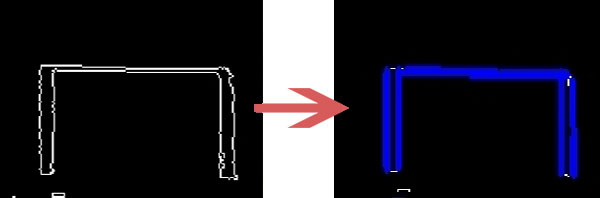
\includegraphics[scale=0.6]{aufspannen.jpg}
\caption{Bild nach Anwendung der Hough-Transformation und dem Aufspannen des Tormodells}
\label{fig:aufspannen}
\end{figure}
\subsubsection{Vorteile der Hough-Transformation an Hand von Beispielen}
Wie zu Beginn erklärt, entstehen Probleme beim Erkennen des Tores z.B. dadurch, dass Teile des Tores verdeckt sind. Dies stellt wie das folgende Beispiel zeigt kein Problem dar. Das Tor wird mittels der Hough-Transformation tortzdem einwandfrei erkannt.
\begin{figure}[H]
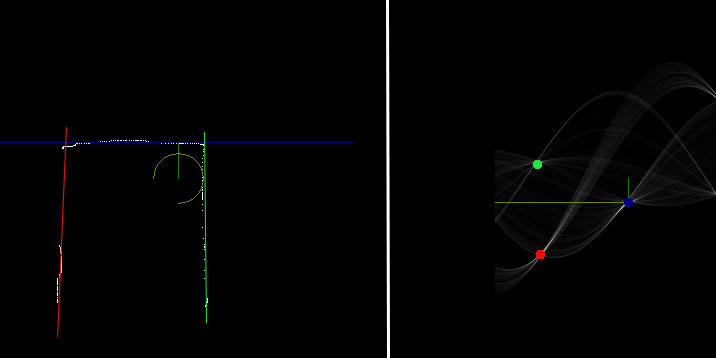
\includegraphics[scale=0.5]{hough_beispiel.jpg}
\caption{Transformation eines Teilweise verdeckten Tores in den Hough-Raum}
\label{fig:houg-beispiel1}
\end{figure}
Abbildung \ref{fig:houg-beispiel1} zeigt wie ein Teilweise verdecktes Tor nach dem Transformieren in den Hough-Raum aussieht, die Häufungspunkte auf der linken Seite sind mit den 3 farbigen Punkten gekennzeichnet und im Ausgansbild sind die farbigen Geraden, die die Punkte repräsentieren eingezeichnet. Man kann sehr schön sehen, dass es kein Problem ist, dass der linke Pfosten nur teilweise zu sehen ist. Der Häufungpunkt wird trotzdem erkannt und der Torpfosten kann komplett modelliert werden. \\
\\
Ein weiteres Problem könnte eine schlechte Perspektive sein. Auch hiermit hat das Verfahren mittels Hough-Transformation keine Probleme. Abbildung \ref{fig:houg-beispiel2} zeigt erneut die Drei Geraden im Ausgansbild mit den zugehörigen Punkten im Hough-Raum farbig markiert. Auch hier ist zu sehen, dass die schlechte Perspektive kein Problem darstellt und das Tor erkannt und modelliert werden kann.
\begin{figure}[H]
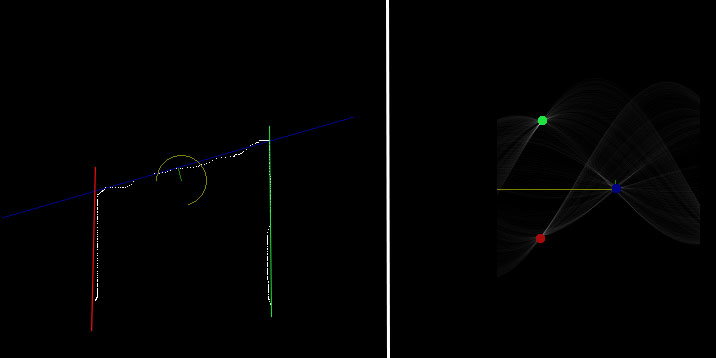
\includegraphics[scale=0.5]{hough_beispiel2.jpg}
\caption{Transformation eines Tores aus einem schlechten Blickwinkel in den Hough-Raum}
\label{fig:houg-beispiel2}
\end{figure}
\section{Fazit}
Das Thema Torerkennung im RoboCup ist und bleibt ein spannendes Thema und wird noch lange einen Schwerpunkt in der Forschung im Bezug auf den RoboCup darstellen. Vor allem die häufigen Regeländerungen machen es erforderlich nahezu jedes Jahr neue Mehtoden zu entwickeln oder alte zu verbessern. Mit zunehmender Verbesserung der Ressourcen wie die Rechenleistung werden auch die Verfahren immer effektiver werden. Man muss Versuchen auf die Eingangs erläuterten Probleme, wie teilweise verdeckte Tore oder den Blick aus einer schlechten Perspektive noch besser lösen. Vor allem aber muss man versuchen den Vorgang der Torerkennung zu beschleunigen.

\newpage
\bibliography{general}
\begin{thebibliography}{9}

  \bibitem{spl-rules}
  Official RoboCup Standard Platform League Rules (http://wiki.robocup.org/wiki/Standard\_Platform\_League\#Rules)
  2010, 2011, 2012.

  \bibitem{humanoid-rules}
  Official RoboCup Humanoid League Rules (http://wiki.robocup.org/wiki/Humanoid\_League\#Rules)
  2009, 2010, 2011, 2012.  

  \bibitem{midsize-rules}
  Official RoboCup Middle Size League Rules (http://wiki.robocup.org/wiki/Middle\_Size\_League\#Rules)
  2009, 2010, 2011, 2012.

  \bibitem{fast-image-seg}
  Fast Image Segmentation, Object Recognition and Localization in a RoboCup Scenario (http://citeseerx.ist.psu.edu/viewdoc/download?doi=10.1.1.27.1388\&rep=rep1\&type=pdf)

  \bibitem{recog-spl}
  Recognition of Standard Platform RoboCup Goals (http://gsyc.es/jmplaza/papers/jopha-2010.pdf)

  \bibitem{yuv}
  YUV-Farbmodell (http://de.wikipedia.org/wiki/YUV-Farbmodell)

  \bibitem{rgb}
  RGB-Farbraum (http://de.wikipedia.org/wiki/RGB-Farbraum)

  \bibitem{hsv}
  HSV-Farbraum (http://de.wikipedia.org/wiki/HSV-Farbraum)

  \bibitem{k-means}
  k-Means-Algorithmus (http://de.wikipedia.org/wiki/K-Means-Algorithmus)
  
  \bibitem{hough}
  Die Hough-Transformation (http://page.mi.fu-berlin.de/alt/vorlesungen/sem04/10\_6Die\%20Hough.doc)
  
  \bibitem{hough2}
  Die Hough-Transformation (http://de.wikipedia.org/wiki/Hough-Transformation)

  \bibitem{hough3}
  Die Hough-Transformation (http://www.malerczyk.de/applets/Hough/Hough.html)
  
  \bibitem{hough4}
  Die Hough-Transformation (http://www.erkenntnishorizont.de/ki/bildverarb/hough.c.php?screen=800)
  
  \bibitem{hough5}
  Hough-Transformation Applett (http://www.activovision.com/octavi/doku.php?id=hough\_transform)
\end{thebibliography}

\end{document}
